
\chapter{OBSERVER BASED CONTROLS}
\label{chap:ObserverBasedControls}

Chapter \ref{chap:UNHTableSat1A} detailed how TableSat's sensor readings could be quantified and represented in terms of engineering units.  Chapter \ref{chap:SatelliteAttitudeDynamicsAndKinematics} established the state representation of the system and the chosen dynamic equations used to model it's behavior.  This chapter will focus on the estimation techniques to improve the accuracy of the state representations, and control techniques to guide the system into the desired state.

\section{Rate and Nutation Estimation Based Control with Sliding Modes}
\label{sec:RateandNutationEstimationBasedControllers}

\TODO{Add explanations}
\begin{figure}[H]
  \centerline{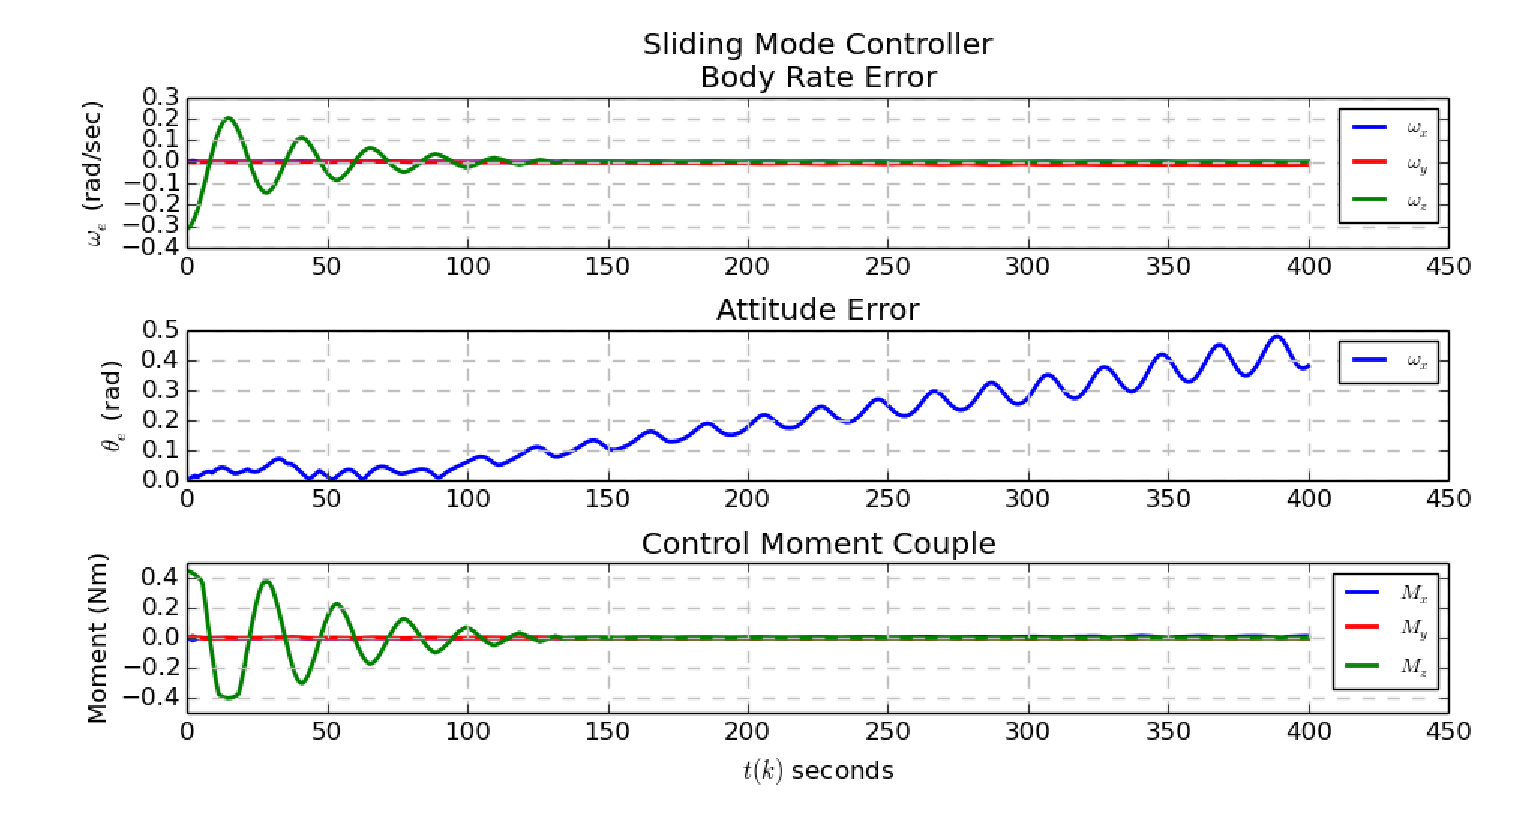
\psfig{file=figures/obc_01_smc.eps,width=6in}}
  \caption{Observer-Based Controller (SMC)}
  \label{fig:ObserverBasedControllerSMC}
\end{figure}

\begin{figure}[H]
  \centerline{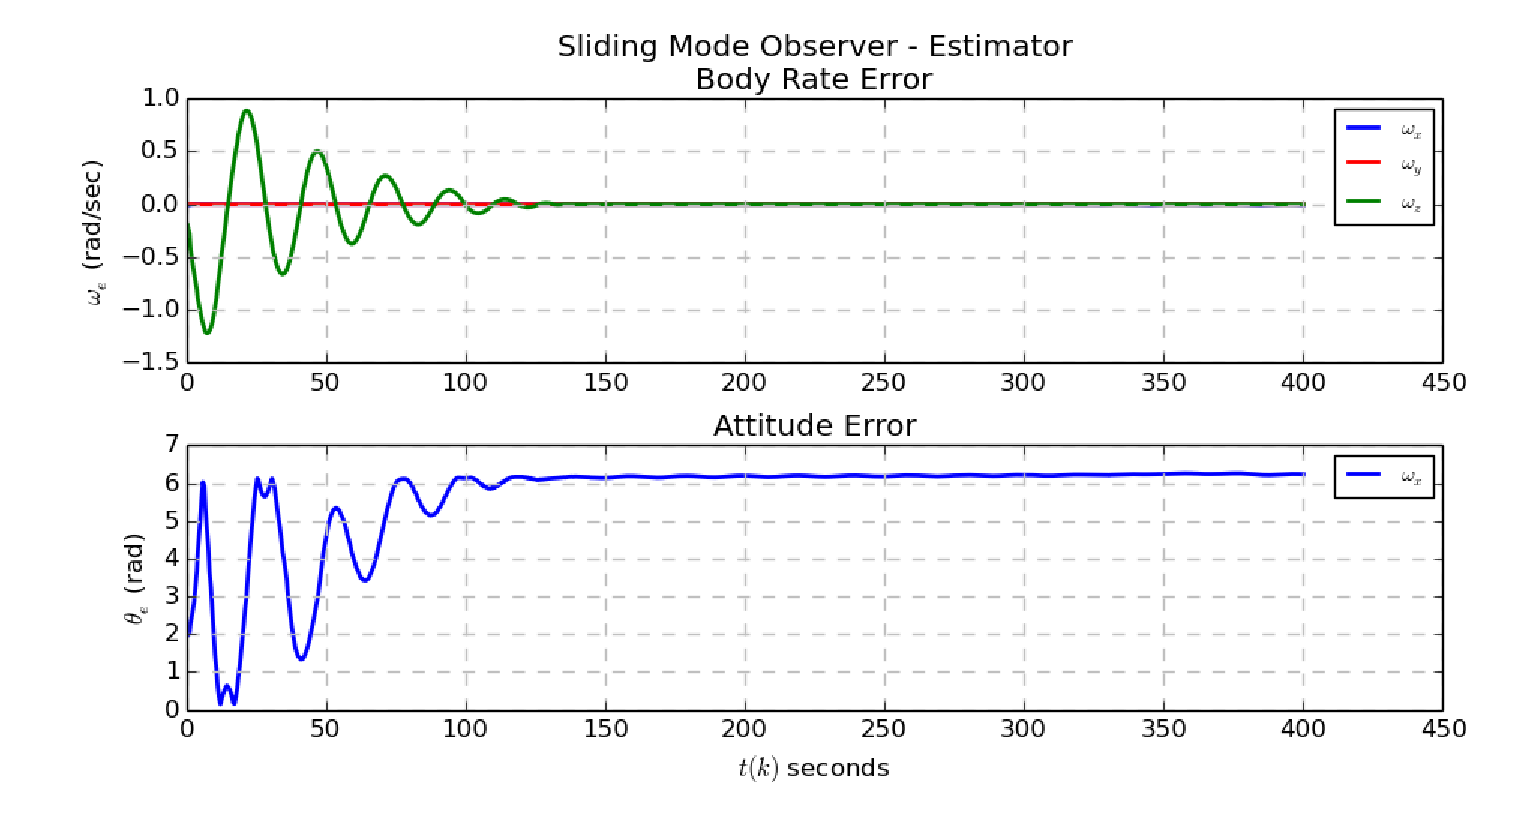
\psfig{file=figures/obc_01_smo.eps,width=6in}}
  \caption{Observer-Based Controller (SMO)}
  \label{fig:ObserverBasedControllerSMO}
\end{figure}

\begin{figure}[H]
  \centerline{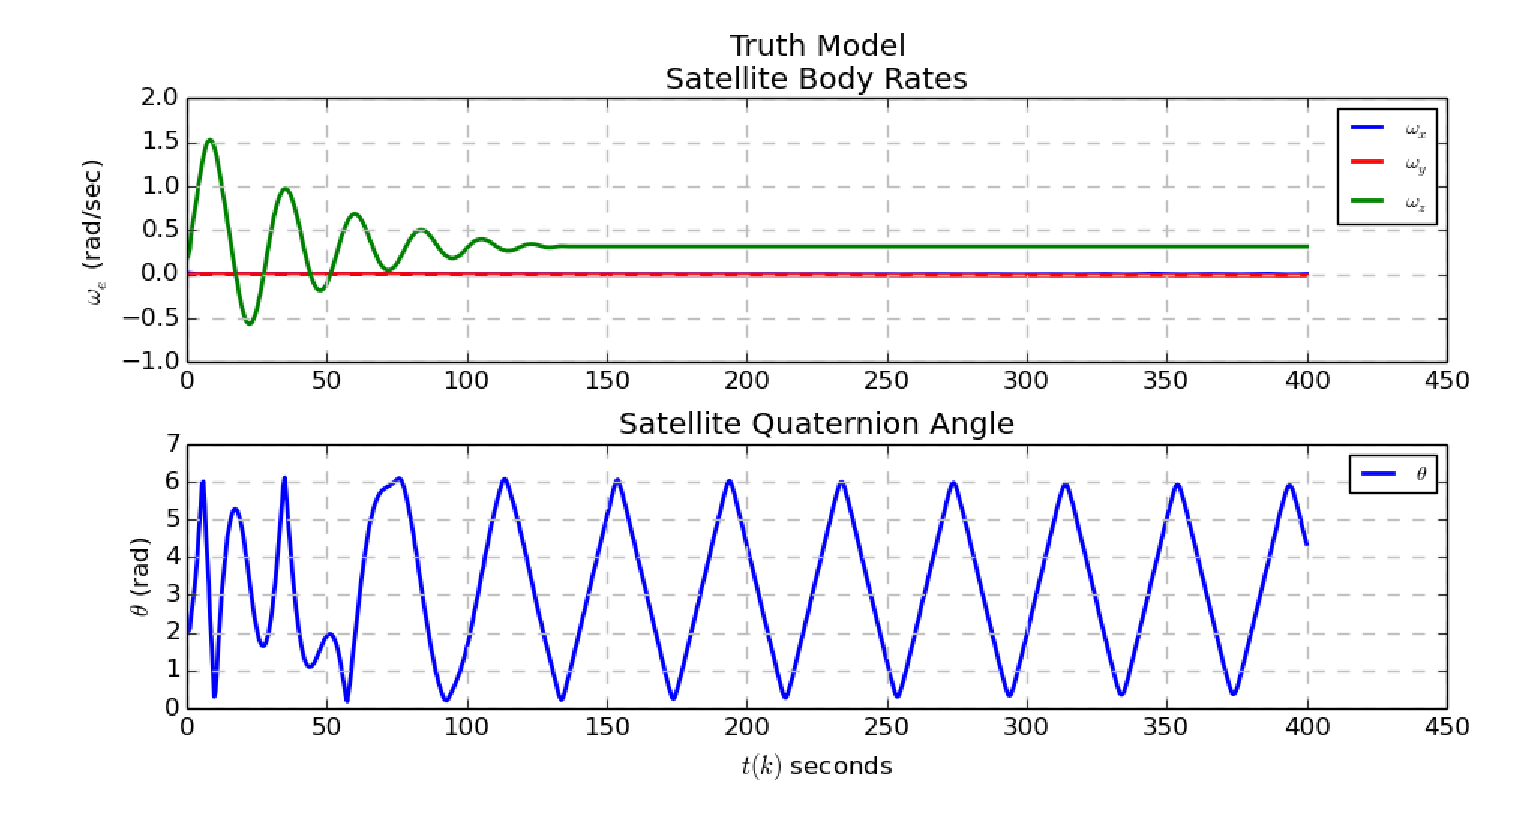
\psfig{file=figures/obc_01_truth.eps,width=6in}}
  \caption{Observer-Based Controller (Truth Model)}
  \label{fig:ObserverBasedControllerTruth}
\end{figure}


\TODO{Adding Noise}
\TODO{Unable to converge with TableSat 1A}

\section{Calculating Nutation From Three-Axis Magnetometer}

\begin{table}[H]
  \centering
  \begin{tabular}{c|ccc|ccc}
    \hline
    Yaw   & & Steady & & & $+X \ 14^o$ & \\ \hline
    (deg) & $TAM_x$ (V) & $TAM_y$ (V) & $TAM_x$ (V) & $TAM_x$ (V) & $TAM_y$ (V) & $TAM_x$ (V)  \\ \hline
    0 & $S_{x0}$ & $S_{y0}$ & $S_{z0}$ & $+X_{x0}$ & $+X_{y0}$ & $+X_{z0}$ \\ \hline
    1 & $S_{x1}$ & $S_{y1}$ & $S_{z1}$ & $+X_{x1}$ & $+X_{y1}$ & $+X_{z1}$ \\ \hline
    ... & & & & & &  \\ \hline
    Yaw   & & $+Y \ 14^o$ & & & $-X \ 14^o$ & \\ \hline
    (deg) & $TAM_x$ (V) & $TAM_y$ (V) & $TAM_x$ (V) & $TAM_x$ (V) & $TAM_y$ (V) & $TAM_x$ (V)  \\ \hline
    0 & $+Y_{x0}$ & $+Y_{y0}$ & $+Y_{z0}$ & $-X_{x0}$ & $-X_{y0}$ & $-X_{z0}$ \\ \hline
    1 & $+Y_{x1}$ & $+Y_{y1}$ & $+Y_{z1}$ & $-X_{x1}$ & $-X_{y1}$ & $-X_{z1}$ \\ \hline
    ... & & & & & &  \\ \hline
    Yaw   & & $-Y \ 14^o$ & &  \\ \hline
    (deg) & $TAM_x$ (V) & $TAM_y$ (V) & $TAM_x$ (V)  \\ \hline
    0 & $-Y_{x0}$ & $-Y_{y0}$ & $-Y_{z0}$  \\ \hline
    1 & $-Y_{x1}$ & $-Y_{y1}$ & $-Y_{z1}$  \\ \hline
    ... & & & & & &  \\ \hline
  \end{tabular}
  \caption{TAM calibration reference table}
  \label{tbl:TAMCalibration}
\end{table}

The following example shows a sample calculation of the nutation based on a single set of coarse sun sensor and TAM voltage measurements.

The base station submits a request for sensor data (message id \#20) to TableSat which responds with a packet contianing the sensor output voltages (message id \#63) with a payload containing 15 floats (timestamp, 6 photodiodes, 4 accelerometrs, gyroscope, and 3 three-axis magnetometer).

\subsection{Calculate Yaw From Coarse Sun Sensor}

Using sample CSS voltages from the photodiodes of 0.37247, 0.30899, 1.18370, 2.40020, 1.80500, and 0.44052.  The TSatPy python package whose development is detailed in Chapter \ref{chap:TSatPy} uses equation \ref{eqn:CSSResultantForce} to convert the sensor voltages into a meaningful state.

\begin{singlespace}
  \begin{minted}[mathescape,
               linenos,
               numbersep=10pt,
               frame=lines,
               framesep=2mm]{python}
import TSatPy
import numpy as np

css_v = [0.37247, 0.30899, 1.18370, 2.40020, 1.80500, 0.44052]

pda = TSatPy.Sensor.PhotoDiodeArray()
pda.update_state(css_v)
vector, radians = pda.x.q.to_rotation()

print "A %g radian (%d degree) rotation about <%g, %g, %g>" % (
    radians, radians / np.pi * 180,
    vector[0,0], vector[1,0], vector[2,0])

# Prints out
# A 3.34585 radian (191 degree) rotation about <-0, -0, -1>
  \end{minted}
  \nocite{minted}
\end{singlespace}

\subsection{Calculate TAM Nutation Reference Data}
\label{subsec:CalculateTAMNutationReferenceData}

Figure \ref{fig:TAMNutationVoltages} shows that while the TAM readings vary enough to be noticeable for large nutations, the signal contain a significant level of noise.  In order to use the TAM to quantify nutation for the observer-based controller, the data in Table \ref{tbl:TAMCalibration} is reduced to five data points for a yaw angle of 191 degrees.  When running the estimator, TAM sensor values can be compared to the five reference nutation points of level, $+x$ down, $+y$ down, $-x$ down, and $-y$ down.

The method chosen for creating the five reference points starts with collecting approximately 2400 data points with corresponding TAM and coarse sun sensor voltage readings.  The voltages for each nutation setting are grouped into 1 degree increments.  Multiple rotations create some overlap in measurements.  The final reference value for each degree is calculated through a weighted average of a specified smoothing window.

Figure \ref{fig:TAMNutationReference} shows the result of the nutation reference values for 5, 15 and 25 degree smoothing windows.  At $\pm 15$ degrees, an adequate level of noise is filtered without causing over smoothing.  At this level, each of the 191 degree reference values are a weighted average of about 200 of the original calibration points.

\begin{figure}[H]
  \begin{subfigure}[h!]{0.5\textwidth}
    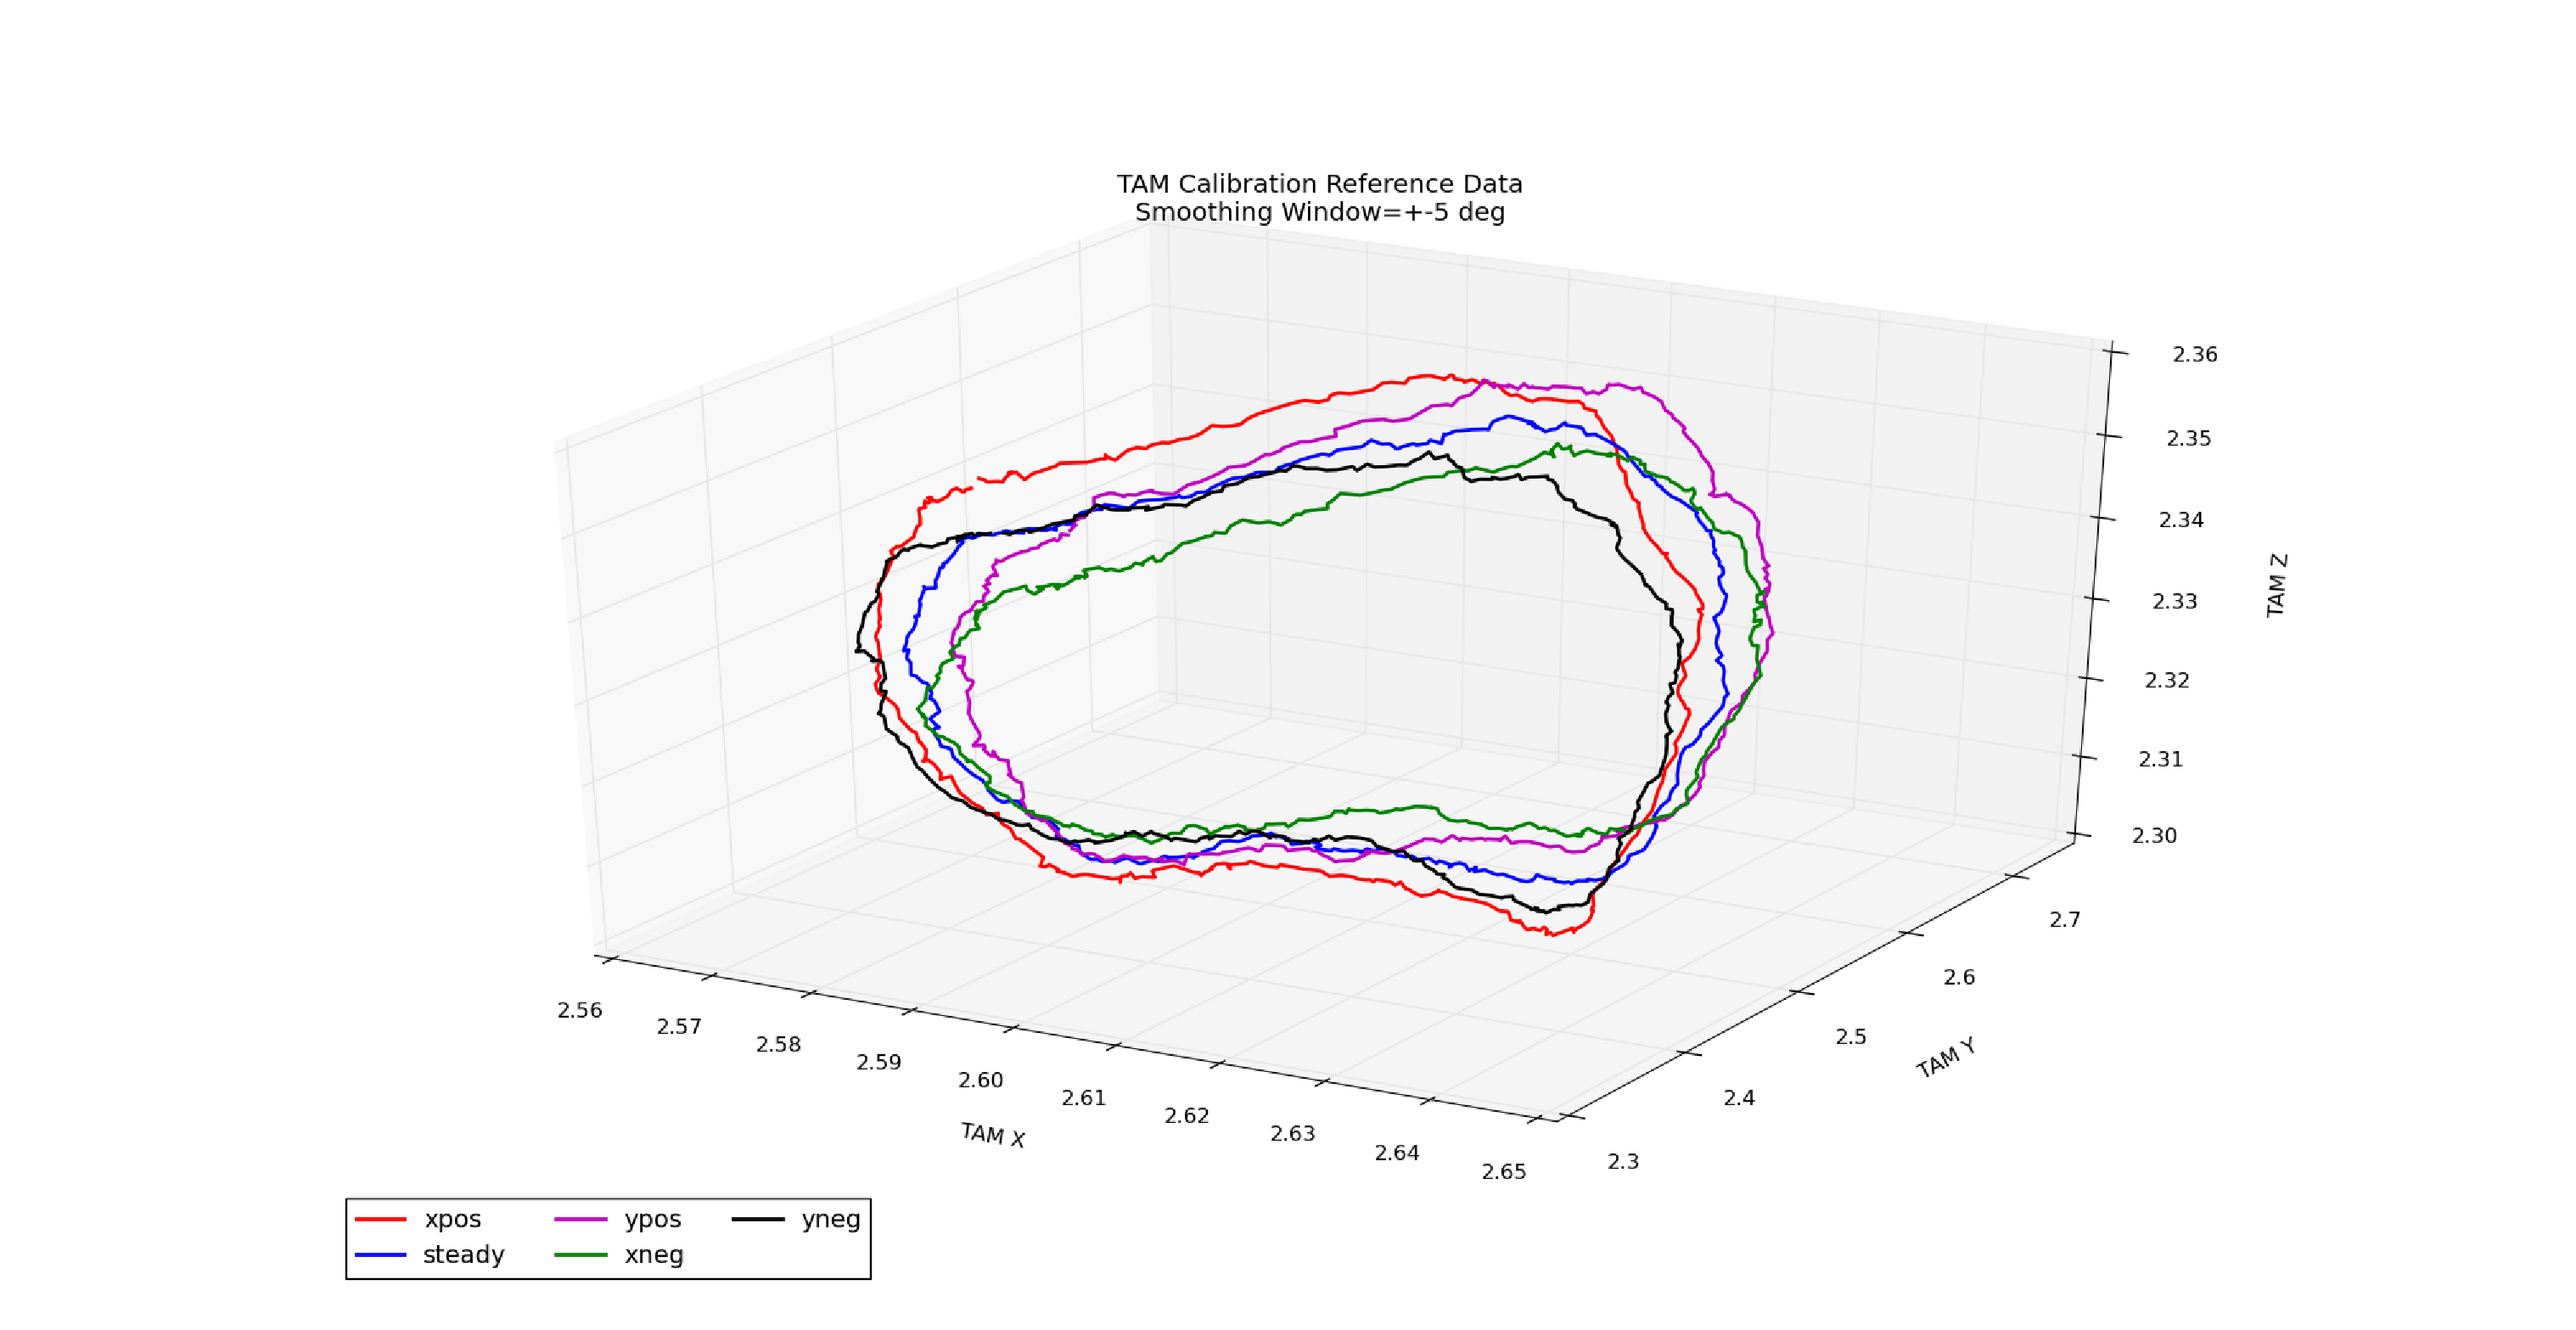
\includegraphics[width=\textwidth]{figures/tam_calibration_ref_5deg_smoothing.eps}
    \caption{$\pm 5^o$ smoothing}
    \label{fig:TAM5degCalibration}
  \end{subfigure}
  ~
  \begin{subfigure}[h!]{0.5\textwidth}
    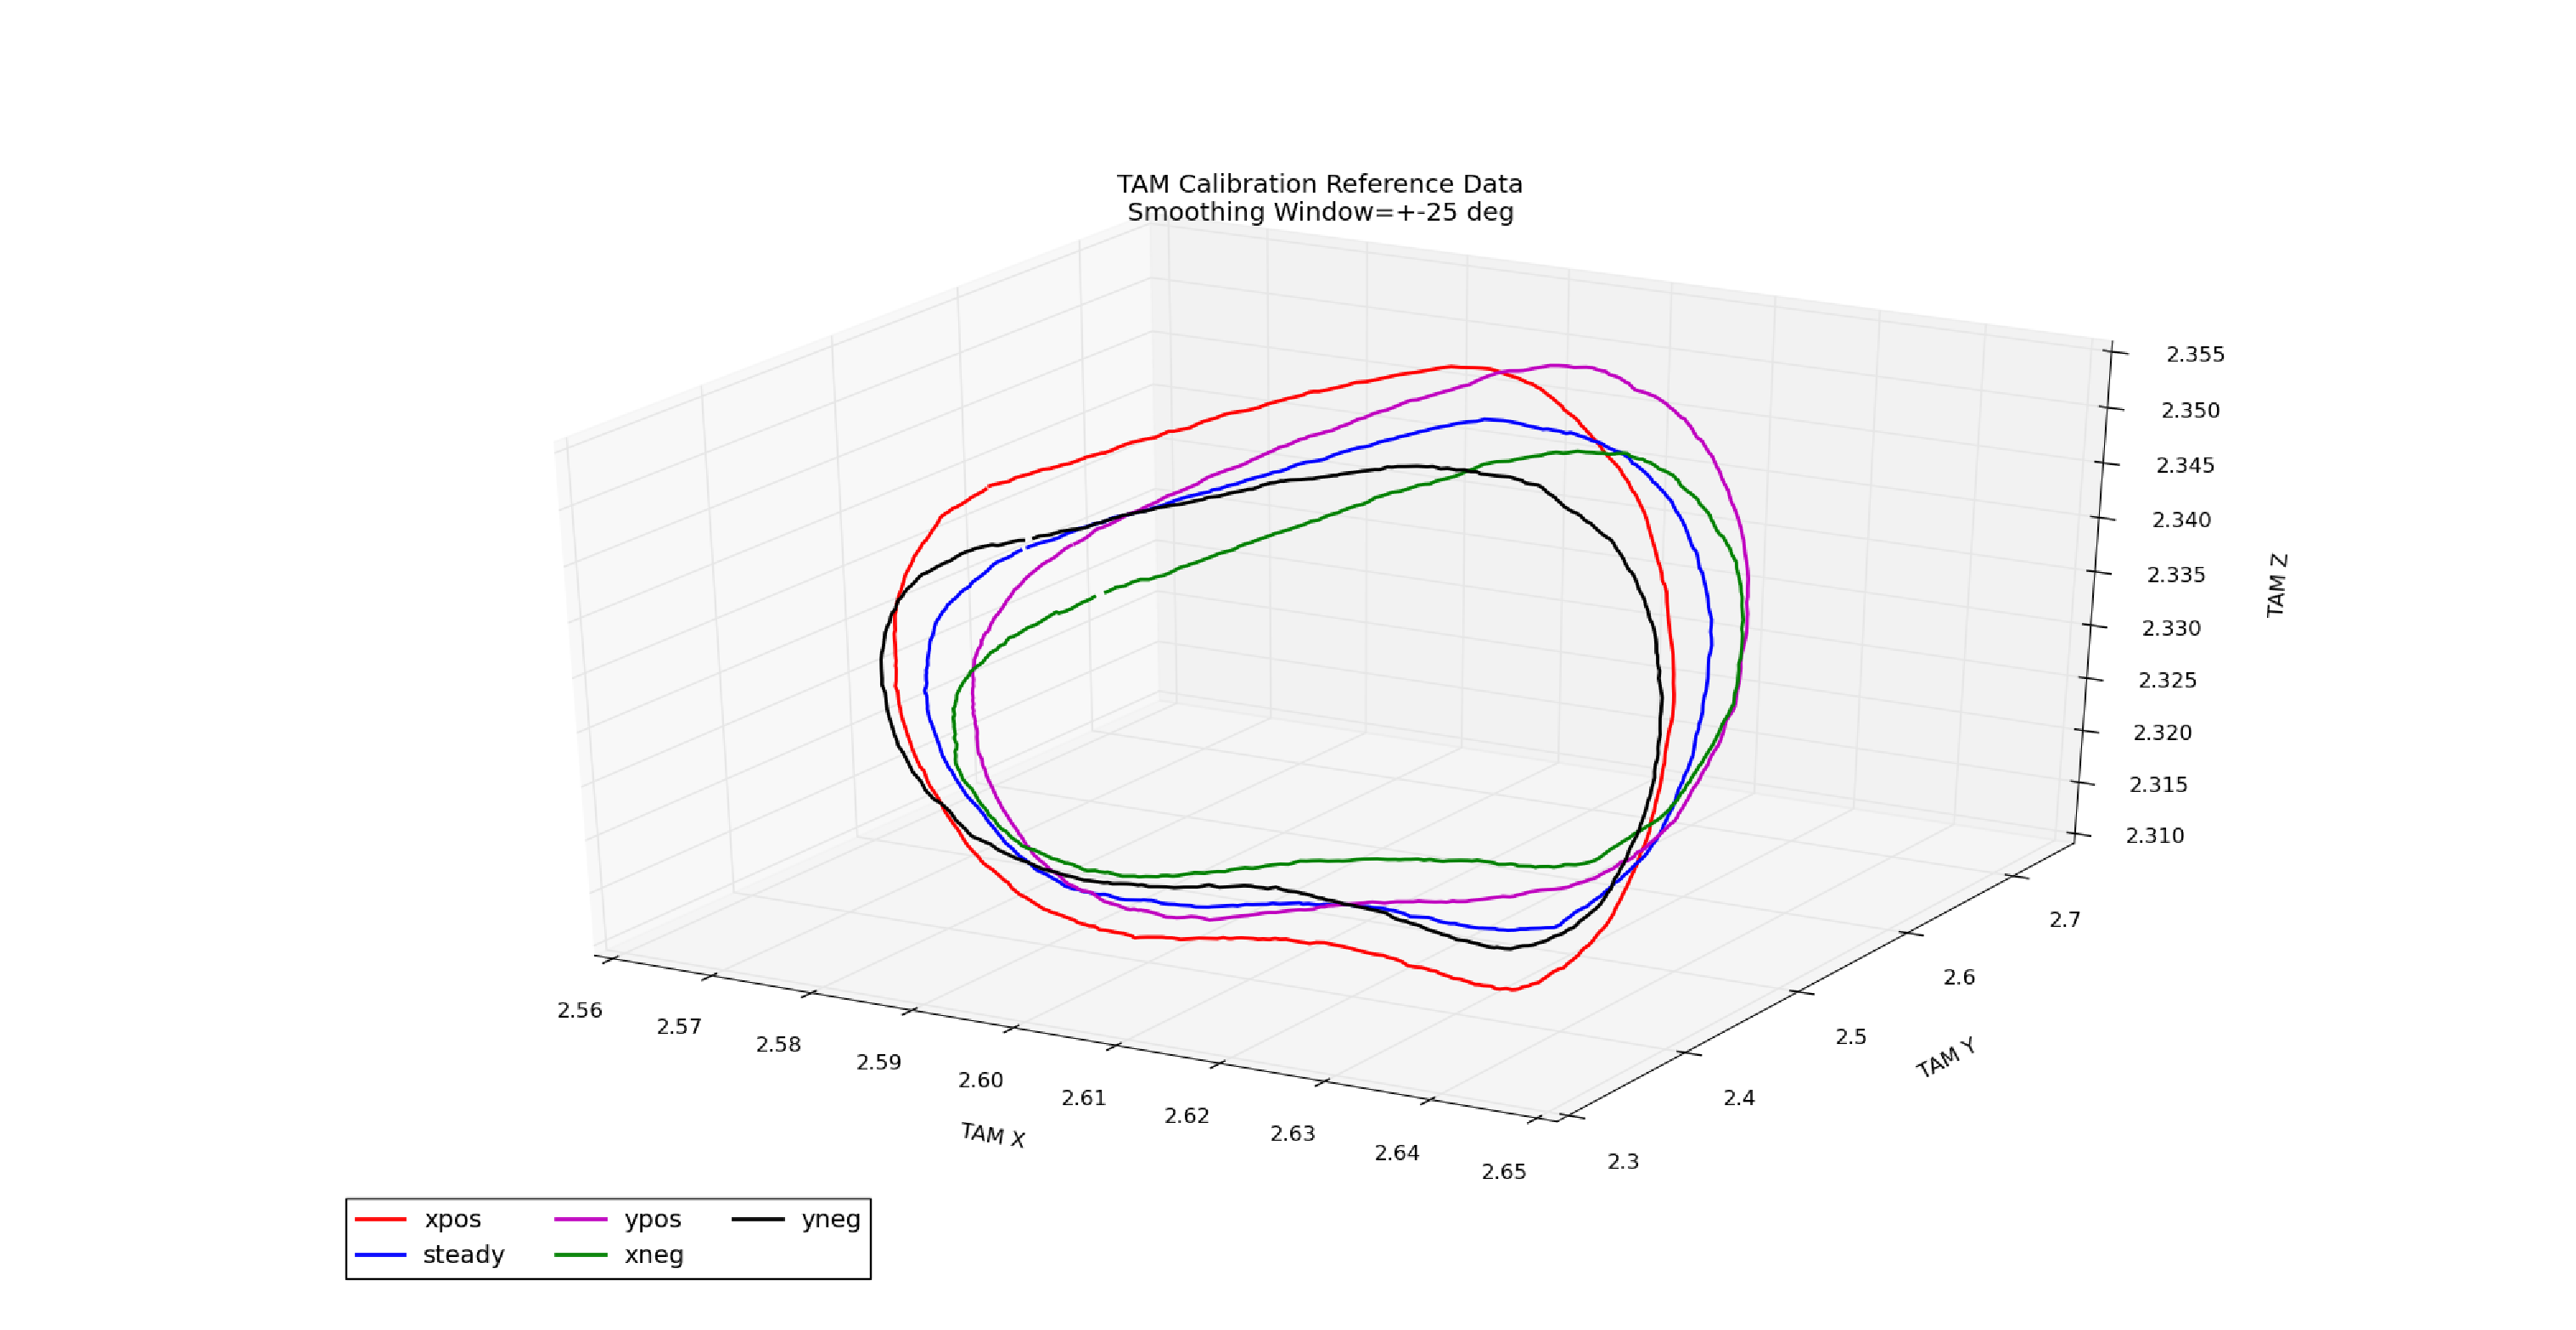
\includegraphics[width=\textwidth]{figures/tam_calibration_ref_25deg_smoothing.eps}
    \caption{$\pm 25^o$ smoothing}
    \label{fig:TAM25degCalibration}
  \end{subfigure}

  \begin{subfigure}[h!]{0.8\textwidth}
    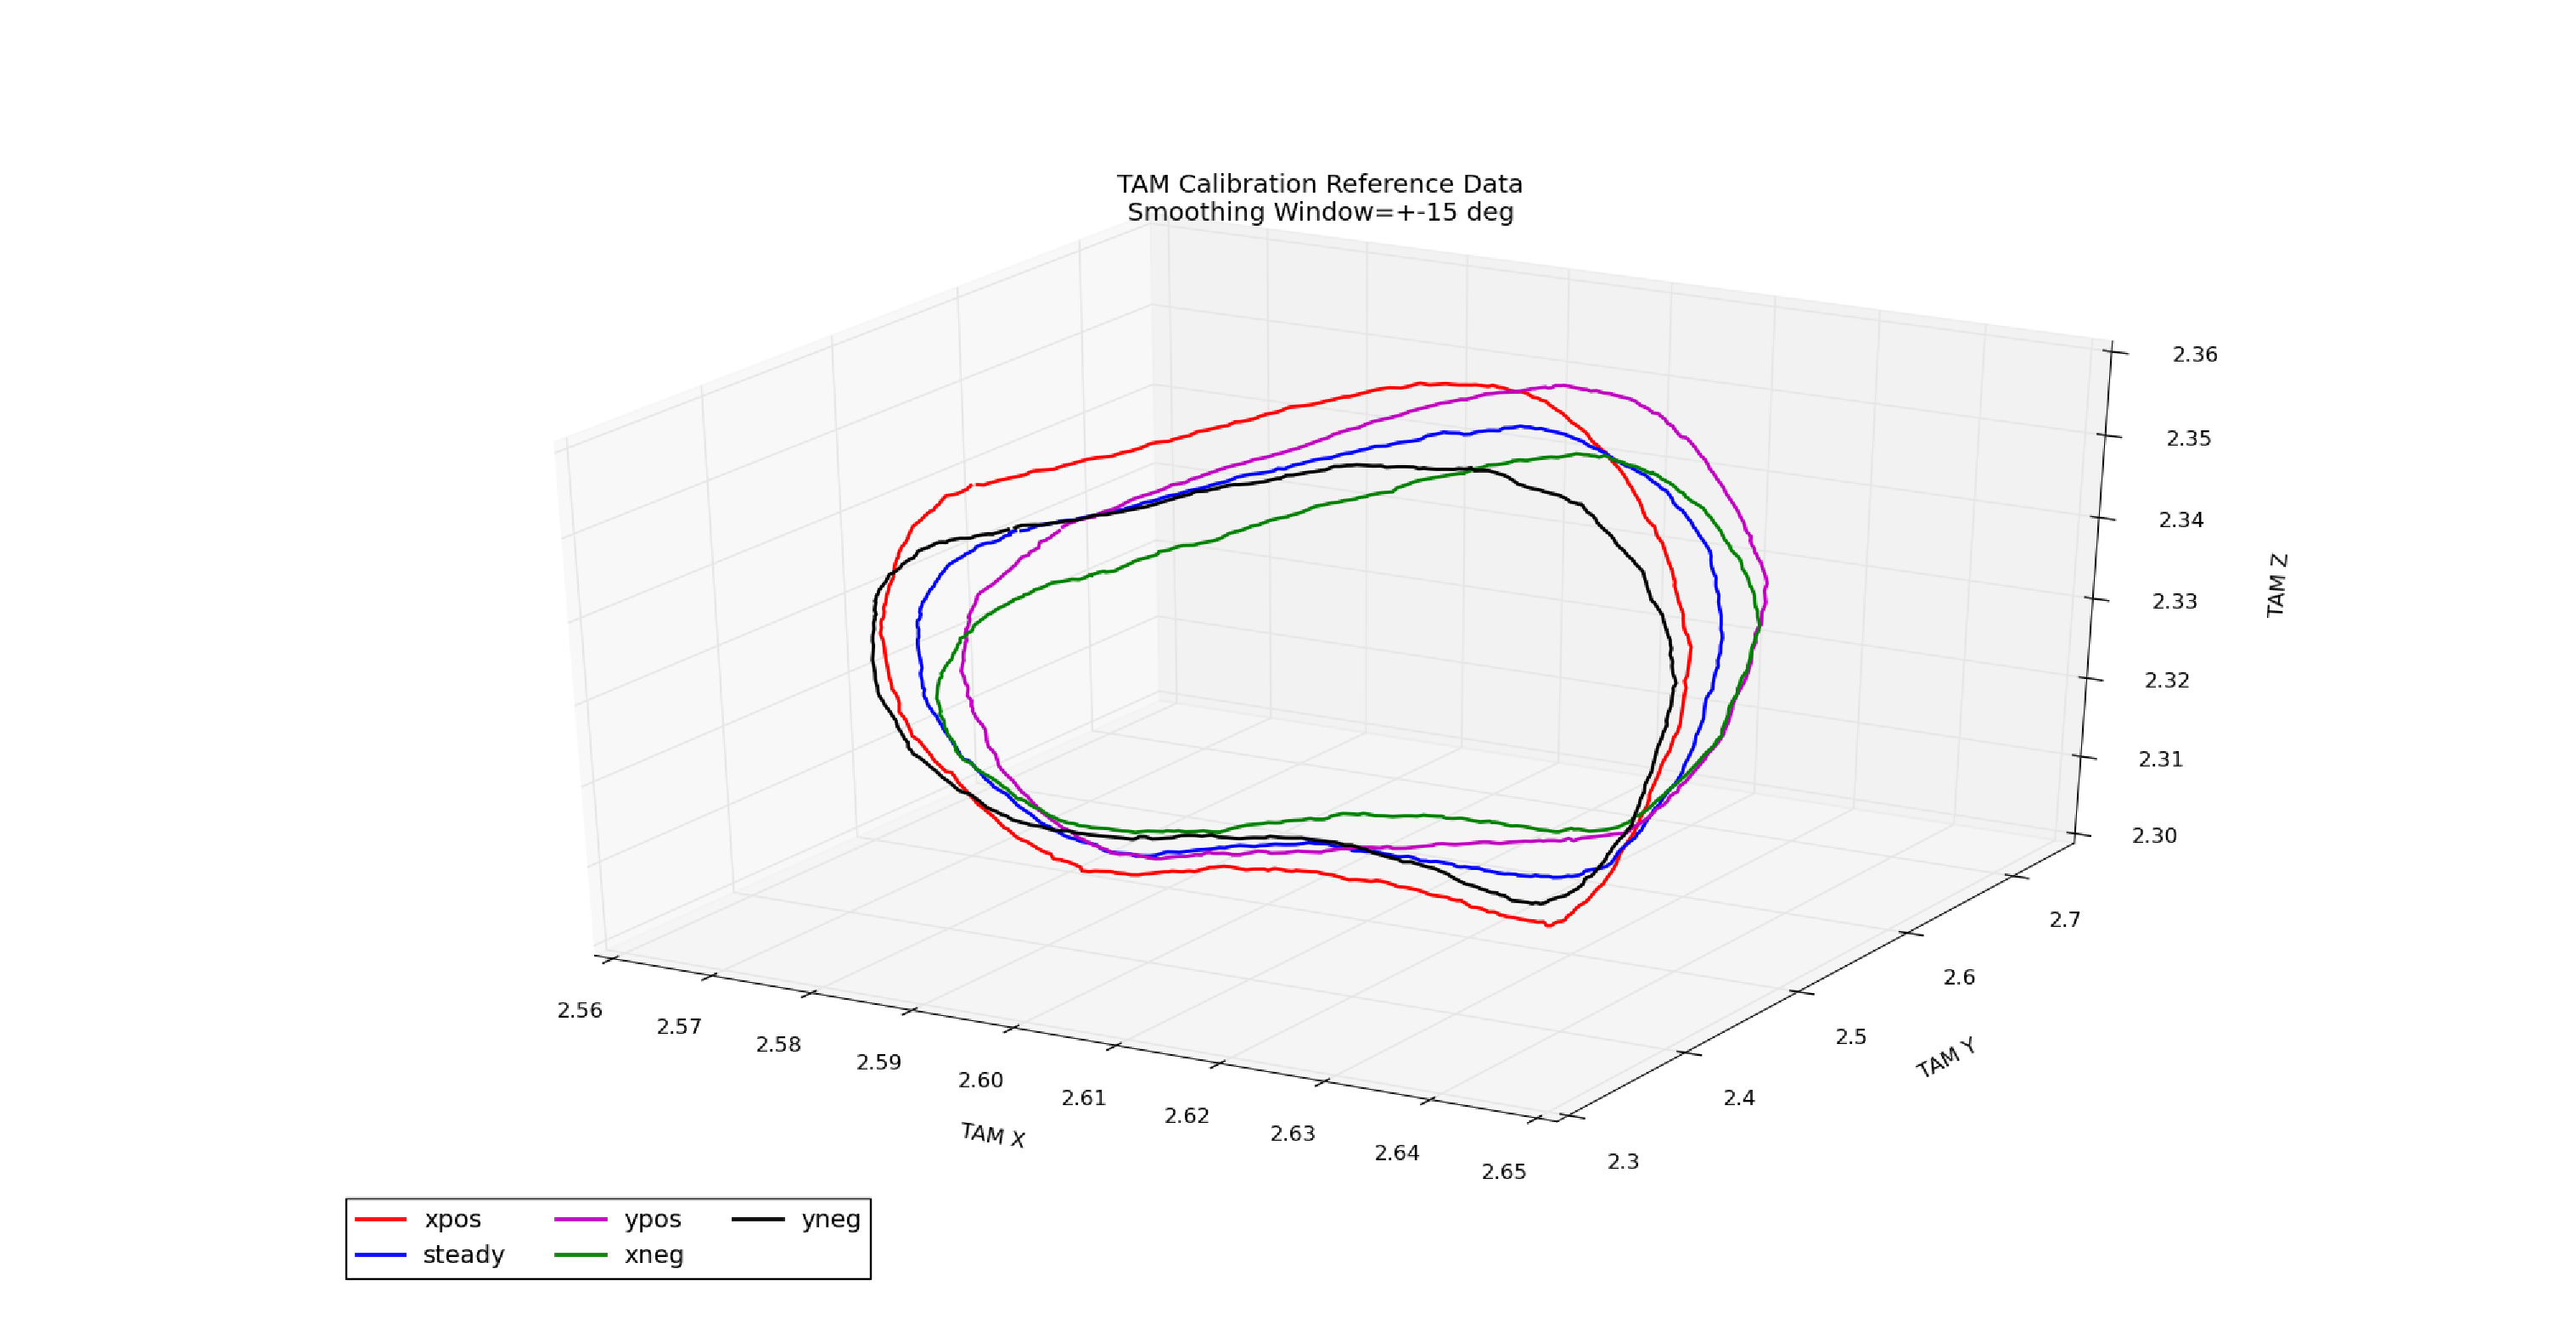
\includegraphics[width=\textwidth]{figures/tam_calibration_ref_15deg_smoothing.eps}
    \caption{$\pm 15^o$ smoothing}
    \label{fig:TAM15degCalibration}
  \end{subfigure}
  \caption{TAM Nutation Reference Values}
  \label{fig:TAMNutationReference}
\end{figure}

The cross shown in Figure \ref{fig:TAMRef191} illustrates the difference in the four nutation reference points compared to the stable point for a 191 degree yaw.  Figure \ref{fig:TAMPoints191} shows the level of noise reduction by the calibration process as the original data points are plotted against the reference nutation voltages.

\begin{figure}[H]
  \centerline{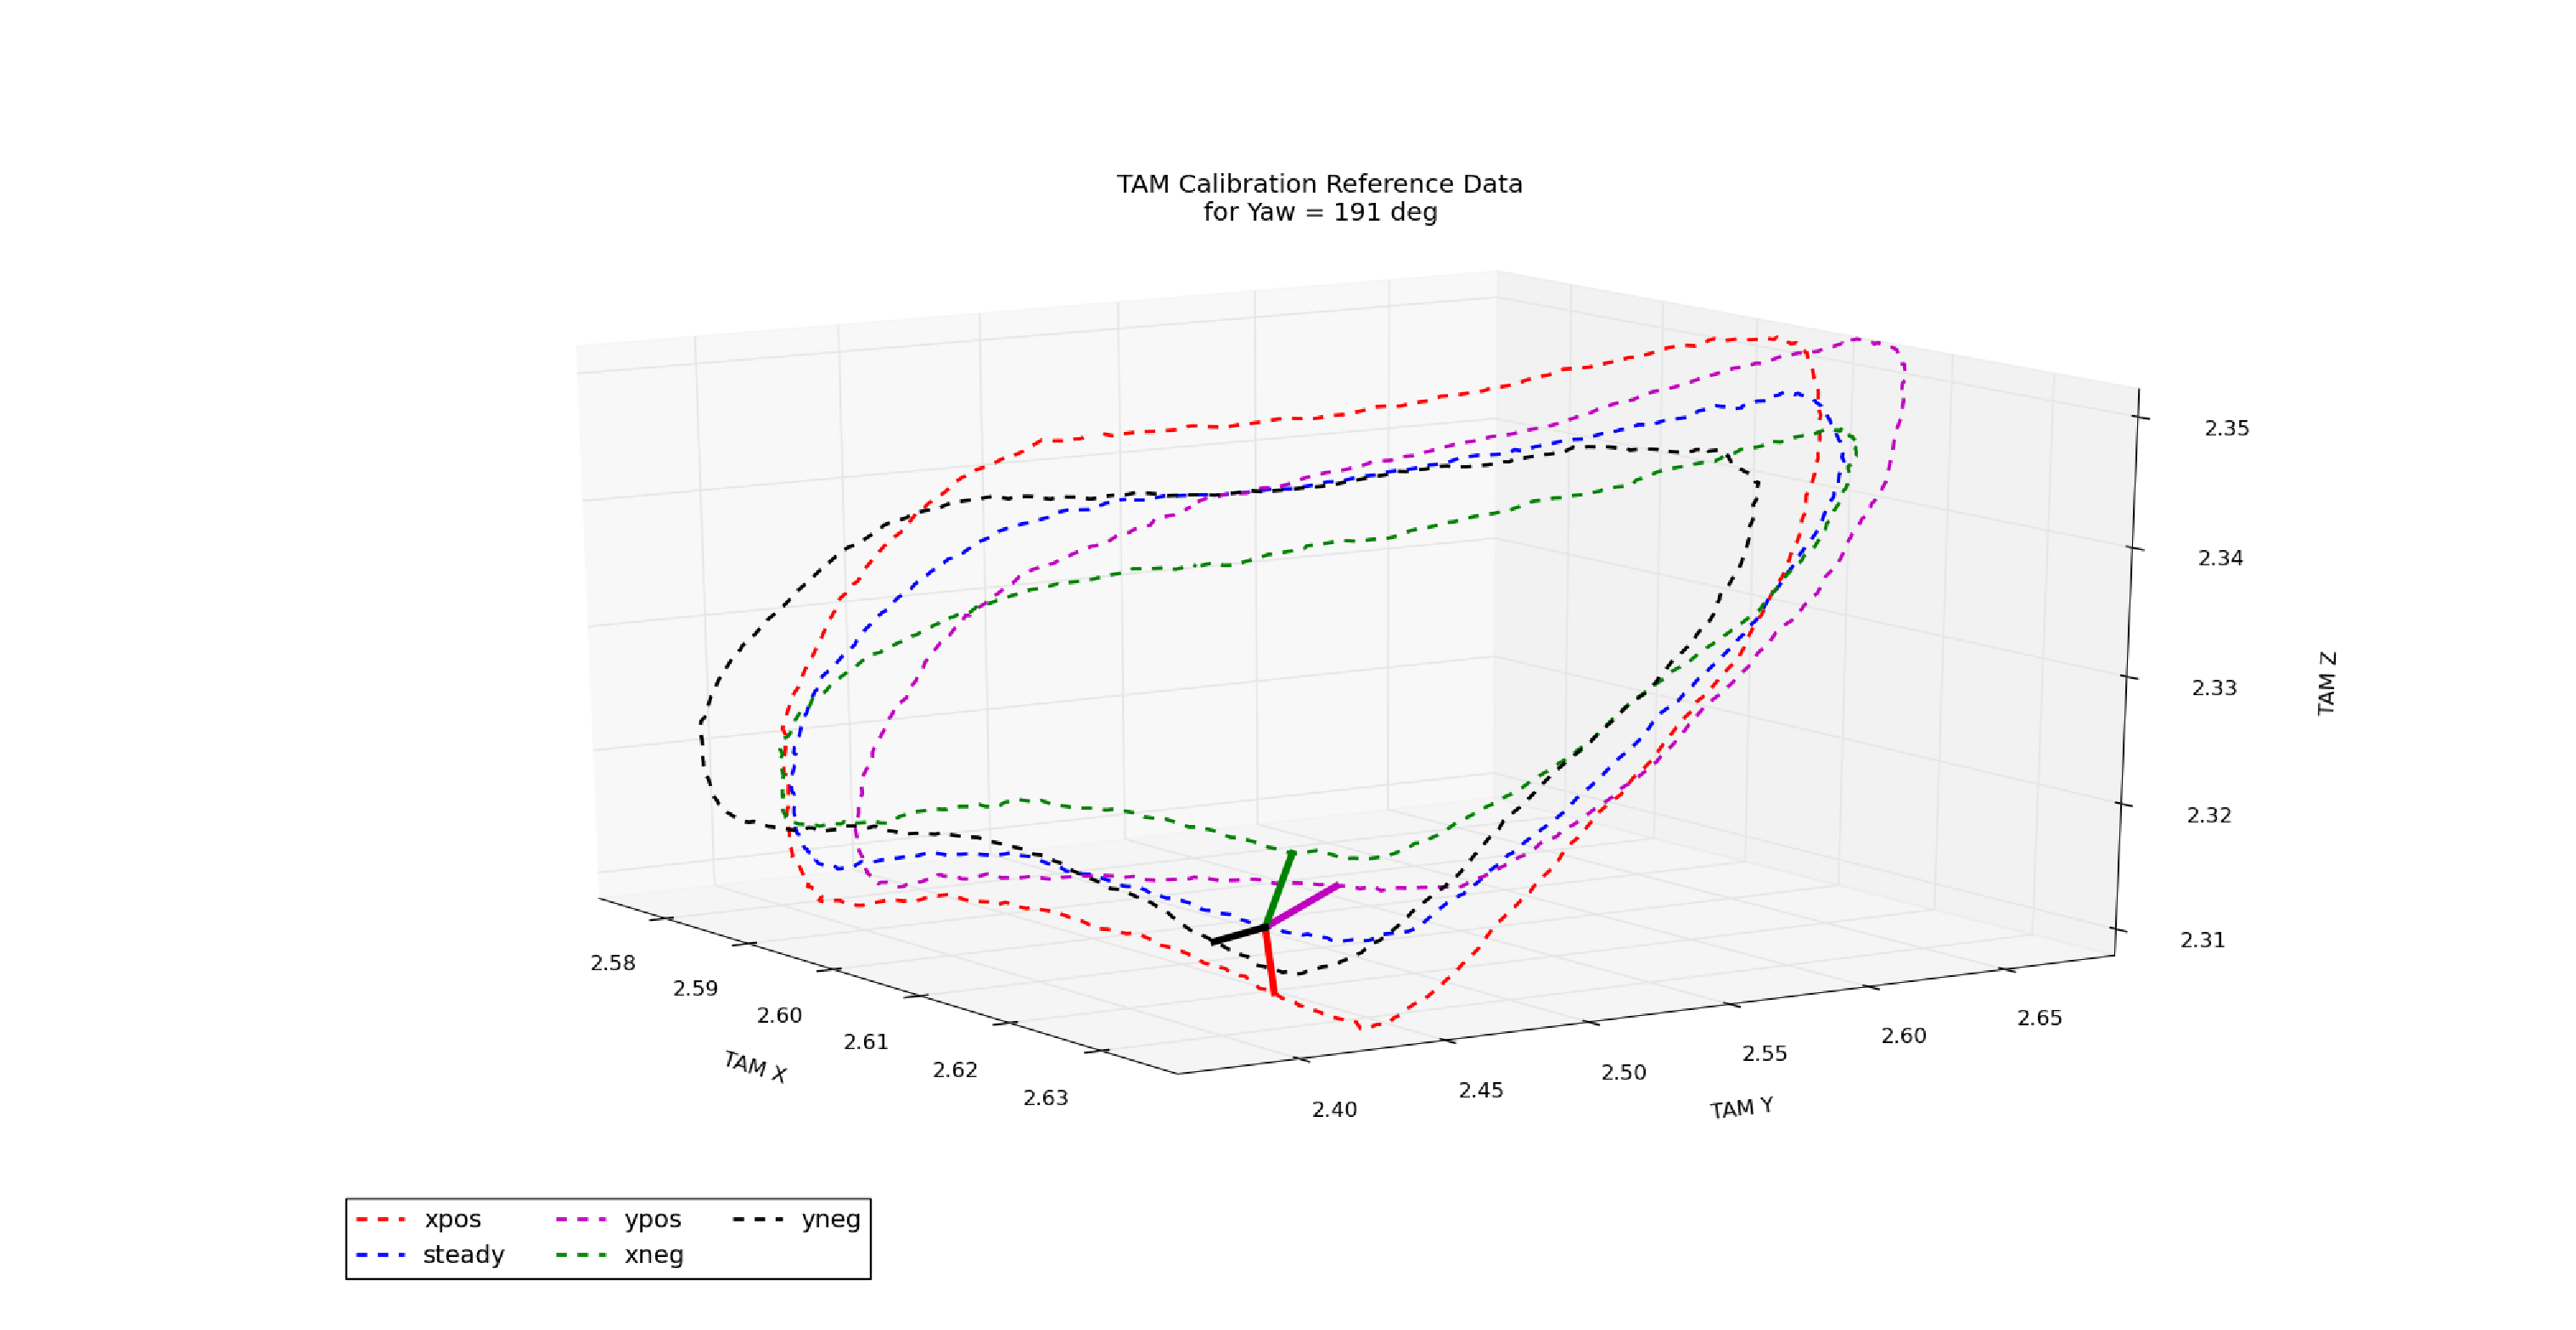
\psfig{file=figures/tam_calibration_ref_for_yaw_191.eps,height=3in}}
  \caption{TAM reference voltages for 191 degree yaw}
  \label{fig:TAMRef191}
\end{figure}

\begin{figure}[H]
  \centerline{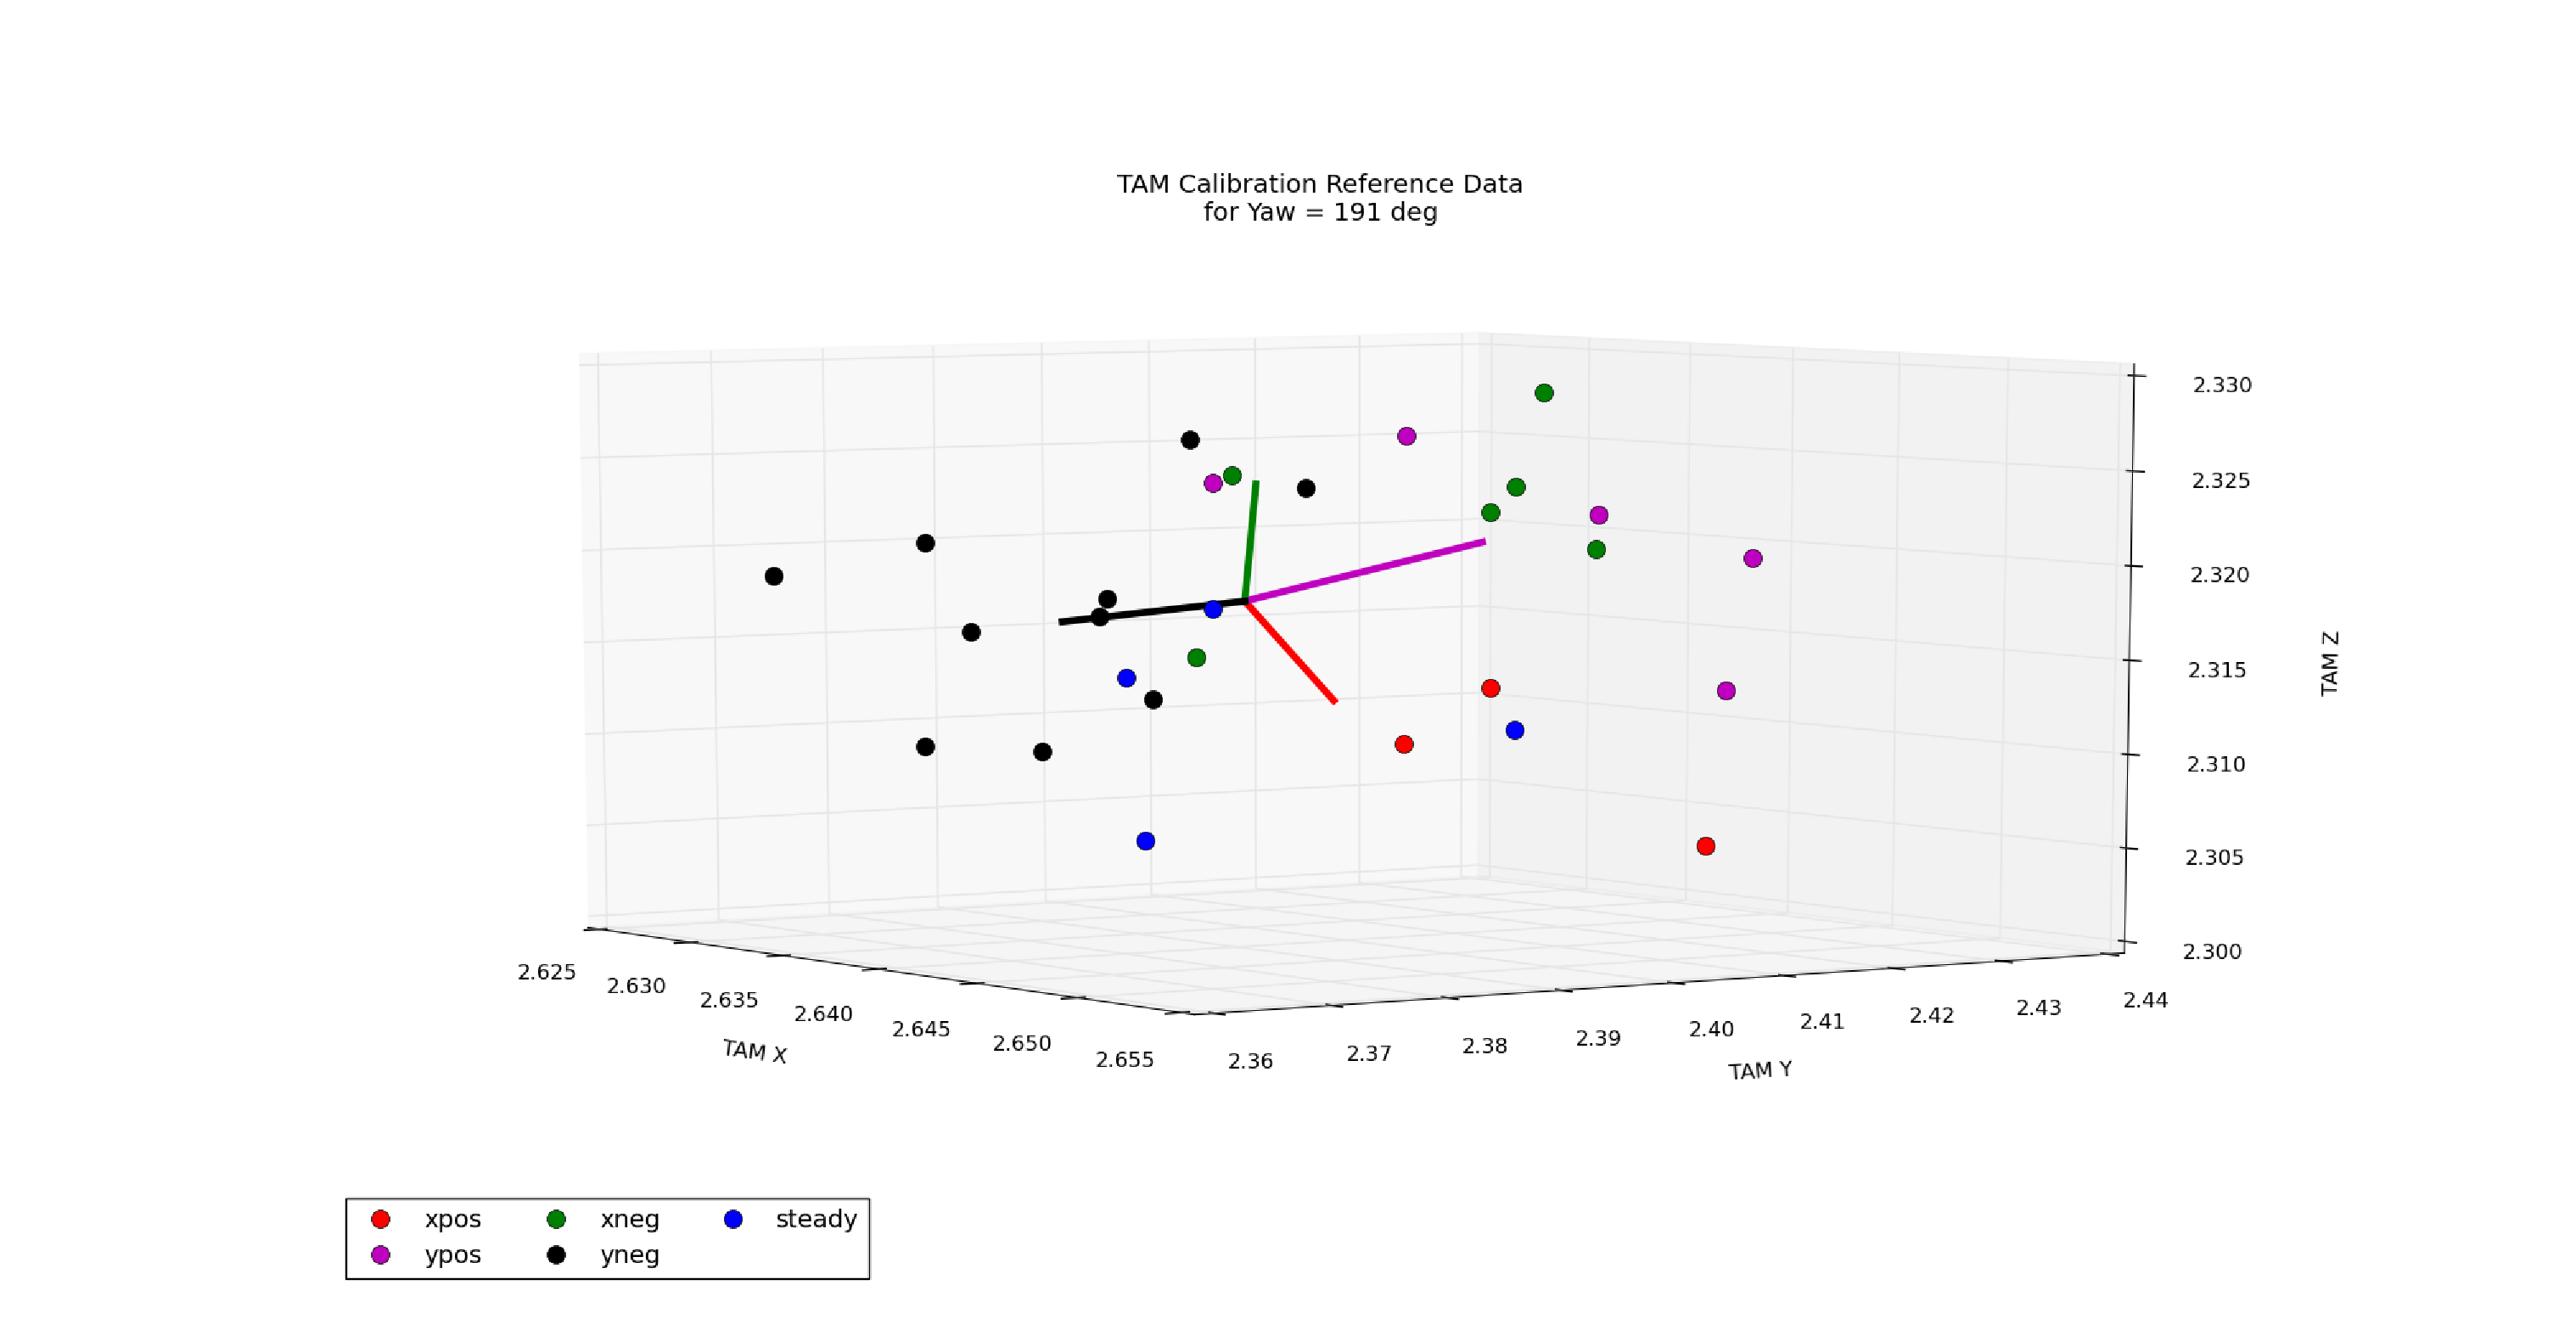
\psfig{file=figures/tam_calibration_191_degree_pts.eps,height=3in}}
  \caption{TAM reference voltages for 191 degree yaw}
  \label{fig:TAMPoints191}
\end{figure}

\subsection{Estimating the Nutation}

Taking one of the points from $-y$ calibration data to complete the example, Table \ref{tbl:TAMSamplePoints} lists the test point, along with the reference values, obtained from the calibration algorithm above.  The test point, plotted in Figure \ref{fig:TAMPoint191} is nearest to the reference $-y$ value, but there is a large gap between the measured value and its associated reference, and other test points as in \ref{fig:TAMPoints191} are far closer to another reference point than its own.

\begin{table}[H]
  \centering
  \begin{tabular}{lc}
    \hline
    Test Point       & $(2.63, 2.37, 2.32)$ \\ \hline
    Steady Reference & $(2.63, 2.40, 2.32)$ \\ \hline
    xpos Reference   & $(2.63, 2.42, 2.31)$ \\ \hline
    ypos Reference   & $(2.64, 2.42, 2.32)$ \\ \hline
    xneg Reference   & $(2.64, 2.39, 2.32)$ \\ \hline
    yneg Reference   & $(2.63, 2.39, 2.32)$ \\ \hline
  \end{tabular}
  \caption{TAM sample reference points}
  \label{tbl:TAMSamplePoints}
\end{table}


\begin{figure}[H]
  \centerline{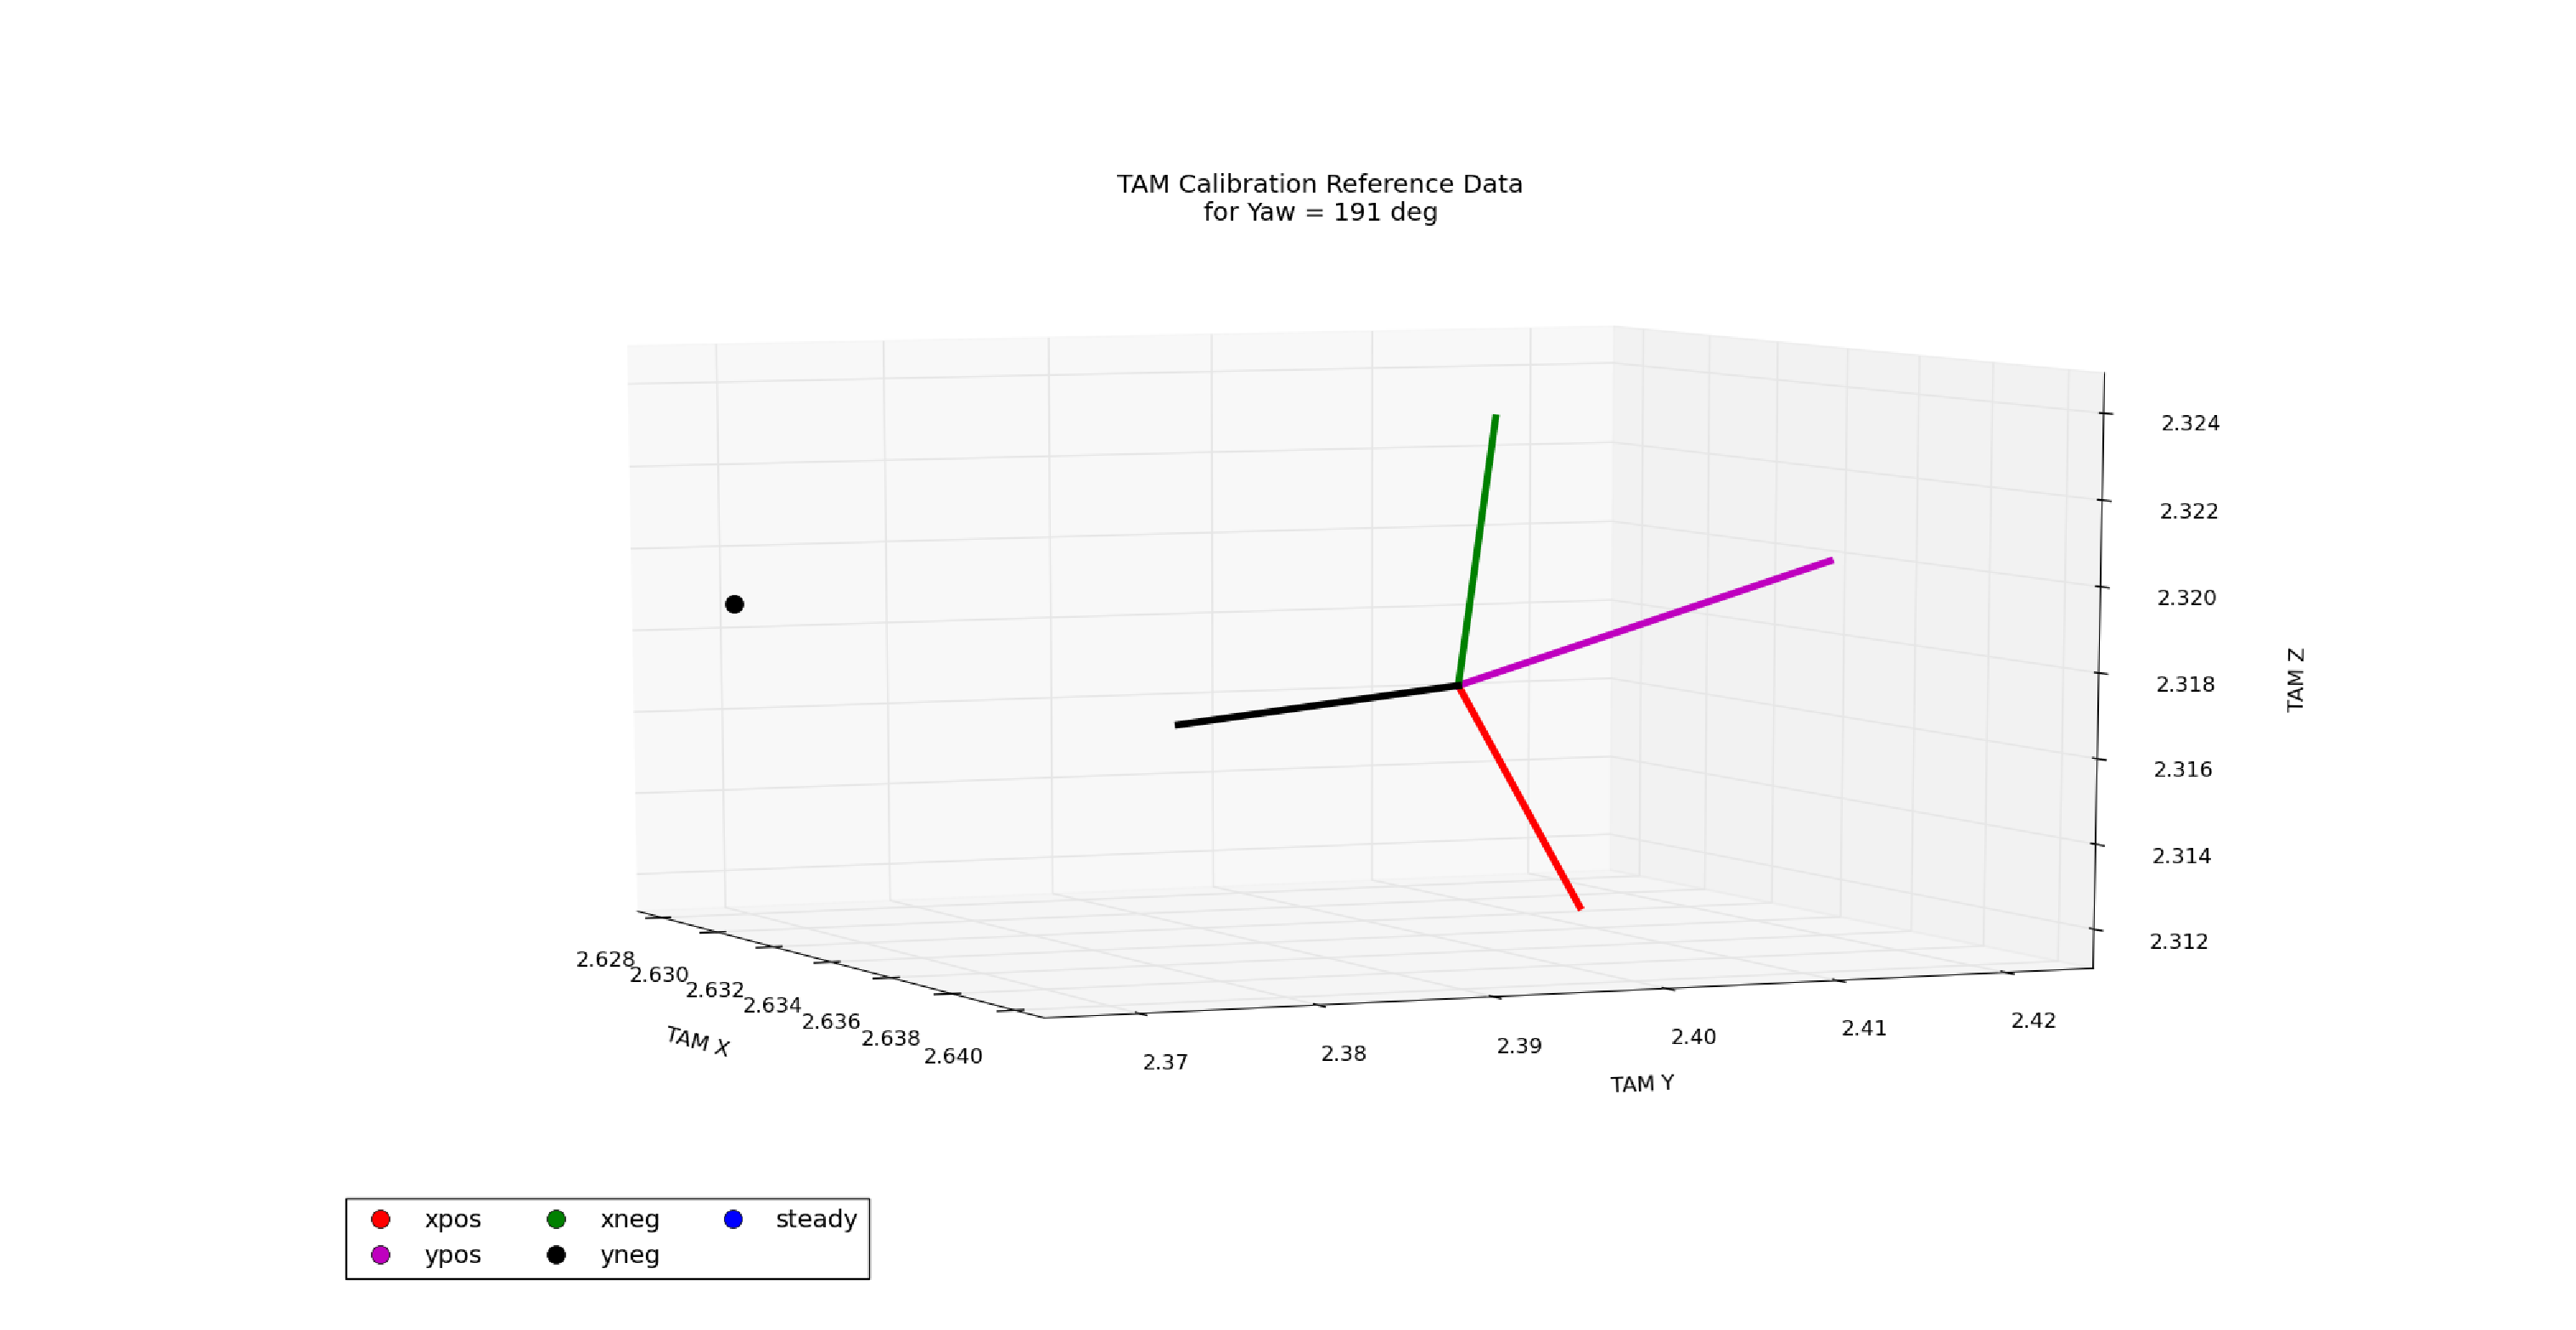
\psfig{file=figures/tam_calibration_191_degree_pt.eps,height=3in}}
  \caption{TAM sample data point for nutation calculation}
  \label{fig:TAMPoint191}
\end{figure}

In order to determine the best approximation for the measured nutations, a number of combinations of approaches are attempted including using the proportion between two estimates, normalizing the reference vectors, projecting the point to the plane consisting of the two nearest vectors, and creating a conversion of the x and y vectors to an orthogonal space.  Some cases provided slightly lower classification error rates when compared to the original calibration test set, but any improvements are not significant.  For simplicity and speed, the measurement estimate for nutation is reduced to a ``nearest neighbor'' classification \cite{nearestneighbor} where the closest reference point is chosen as the best approximation.

Despite the improved speed and simplicity, this classification method has some large faults, the biggest of which is the resulting chattered signal that is relayed to the estimator state.  This is because there are no continuum of values, the nutation state jumps between the five calibration states of level, and each of the $14^o$ nutations.  Further work is needed to refine this technique.
